\chapter{基于技术探针的用户研究}

% 介绍为什么要做这个
日常健康场景与诊所的标准环境相比,场景更加复杂,用户真实想法难以获取,以往的面诊系统研究在交互设计上未能较好地处理这个问题。
为了研究日常使用场景下面诊技术的应用可能会遇到的问题,本文使用了人机交互中基于技术探针的设计方法:本文实现了云中医应用作为技术探针并设计了实验,通过分析访谈数据来探索和总结面诊应用在日常健康场景下的特点和存在的挑战,并给出了对应的设计策略以指导未来的日常场景下面诊系统实现。

\section{技术探针实现:云中医应用}

% 云中医智能镜\cite{李雪2017}是复旦大学计算机学院张文强老师和上海中医药大学合作开发的一款智能产品,旨在为用户提供一个方便的自我诊断和健康管理平台,目前主要应用场景是各大社区、诊所给用户做健康参考。
% 虽然云中医智能镜并不适合在日常场景下使用,但它提供了基于的面诊功能,满足作为技术探针的基于条件。
% 基于云中医智能镜,
本文使用了在上一章提到的人脸检测、唇部舌部区域提取、SVM分类器、诊断规则等方法,开发了一个用于研究日常场景的技术探针:云中医应用。

\begin{figure}[htb]
    \centering
    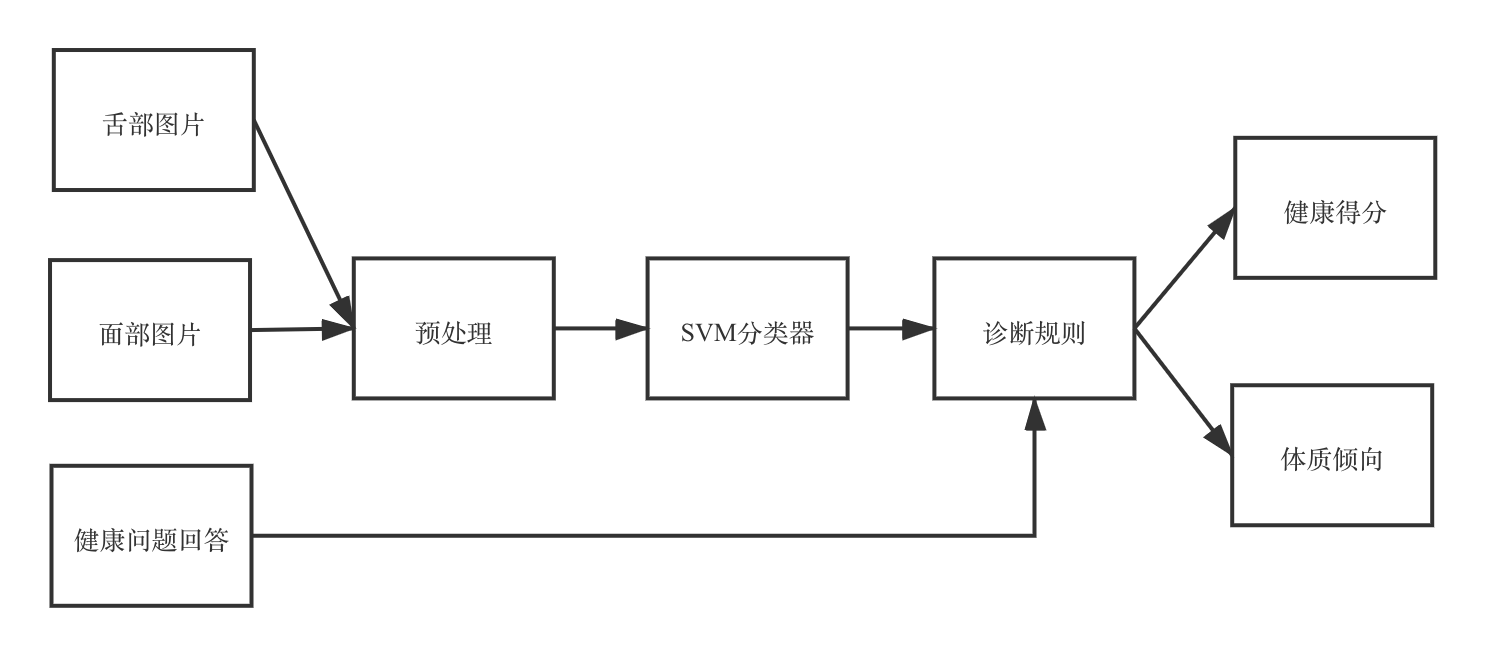
\includegraphics[width=15cm]{images/cloud_med.png}
    \caption{云中医模型处理流程}
    \label{cloudmed}
\end{figure}

云中医应用以中医面诊、舌诊、问诊理论为指导,在手机上目前已经模拟了与目前市面上大部分面诊系统类似的诊断的过程:
用户需要依次对自己的面部和舌头进行拍照,回答一些与自己健康状况相关的问题,最终会收到一份完整的健康报告和一些健康建议。

模型处理流程如图\ref{cloudmed}所示,面部图片、舌部图片和用户对健康问题的回答作为模型输入,经过人脸检测、区域提取算法将图片进行预处理,截取肤色、唇部、舌部区域,通过由人工标记数据训练过的SVM分类器得到更加细粒度的特征。
最后由专家编写的诊断规则将上述过程得到的特征和用户对健康问题的回答,得出用户的健康得分和体质倾向。 

\begin{figure}[htb]
    \centering
    \subfigure[主界面]{
        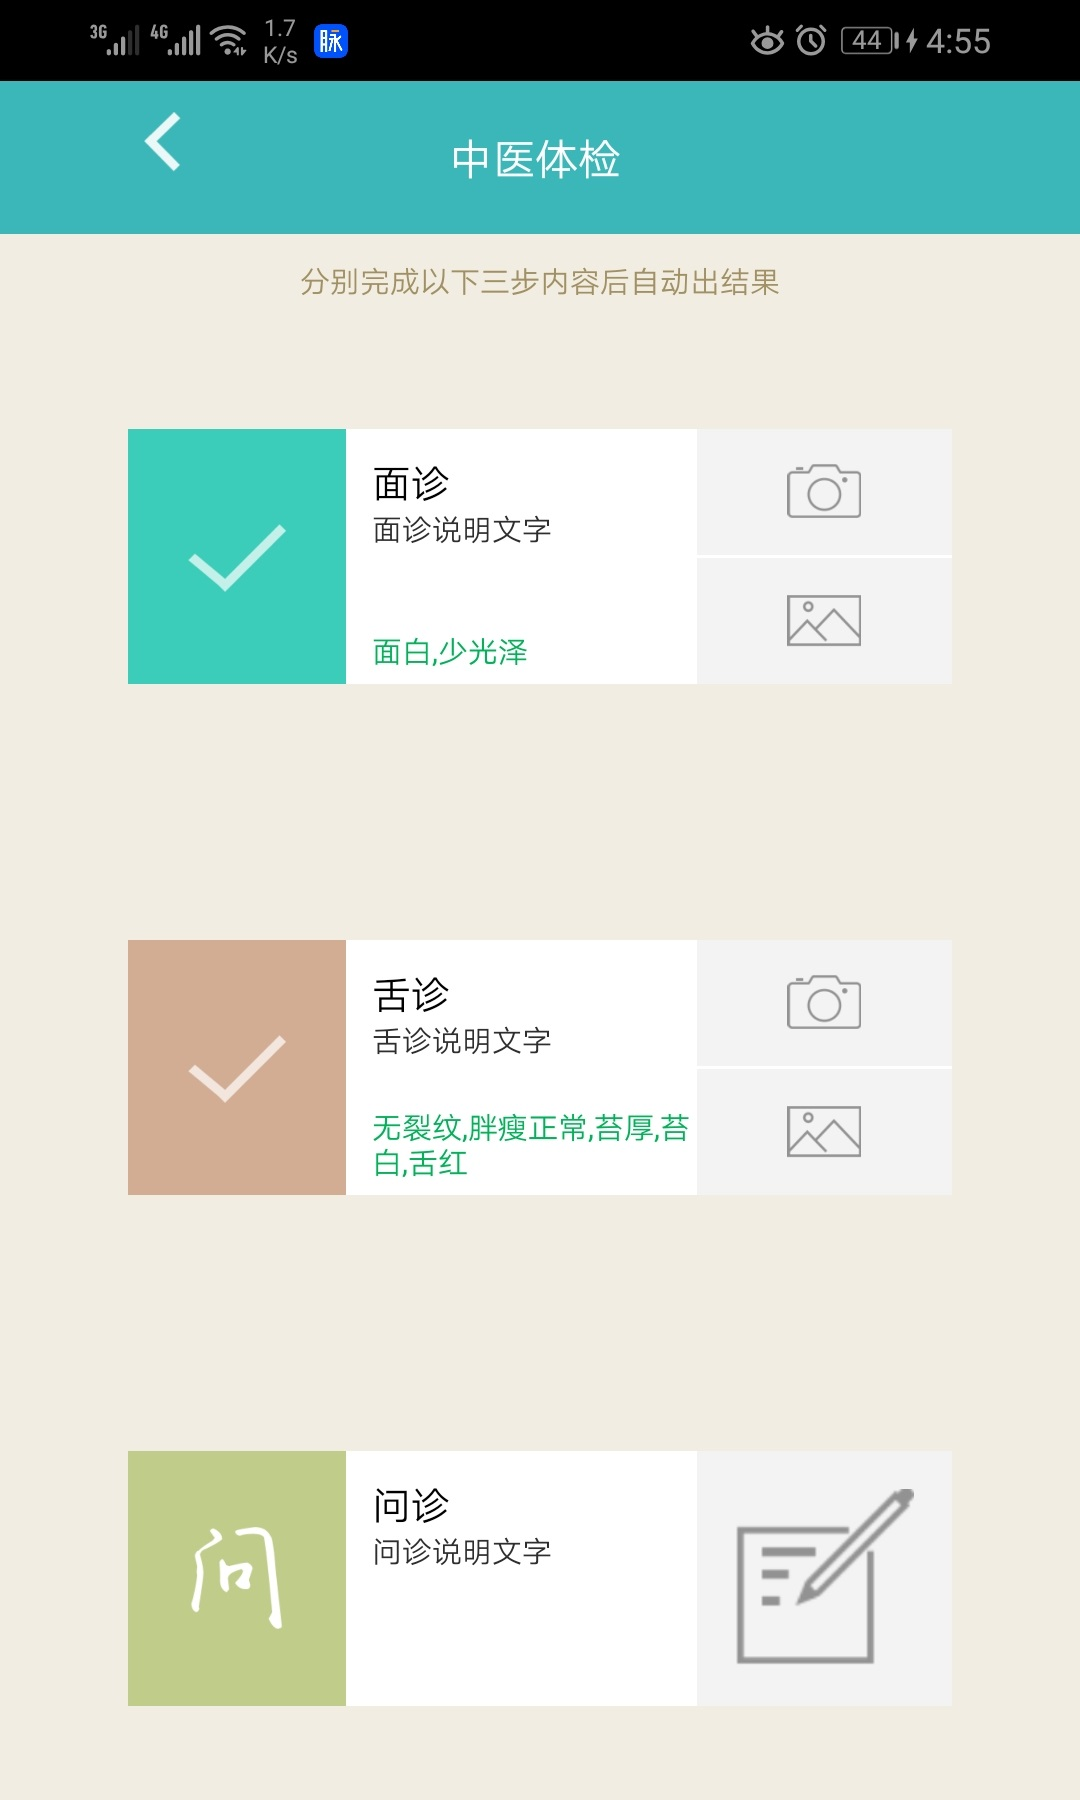
\includegraphics[width=4.5cm]{images/main1.jpg}
    }
    \subfigure[问诊]{
        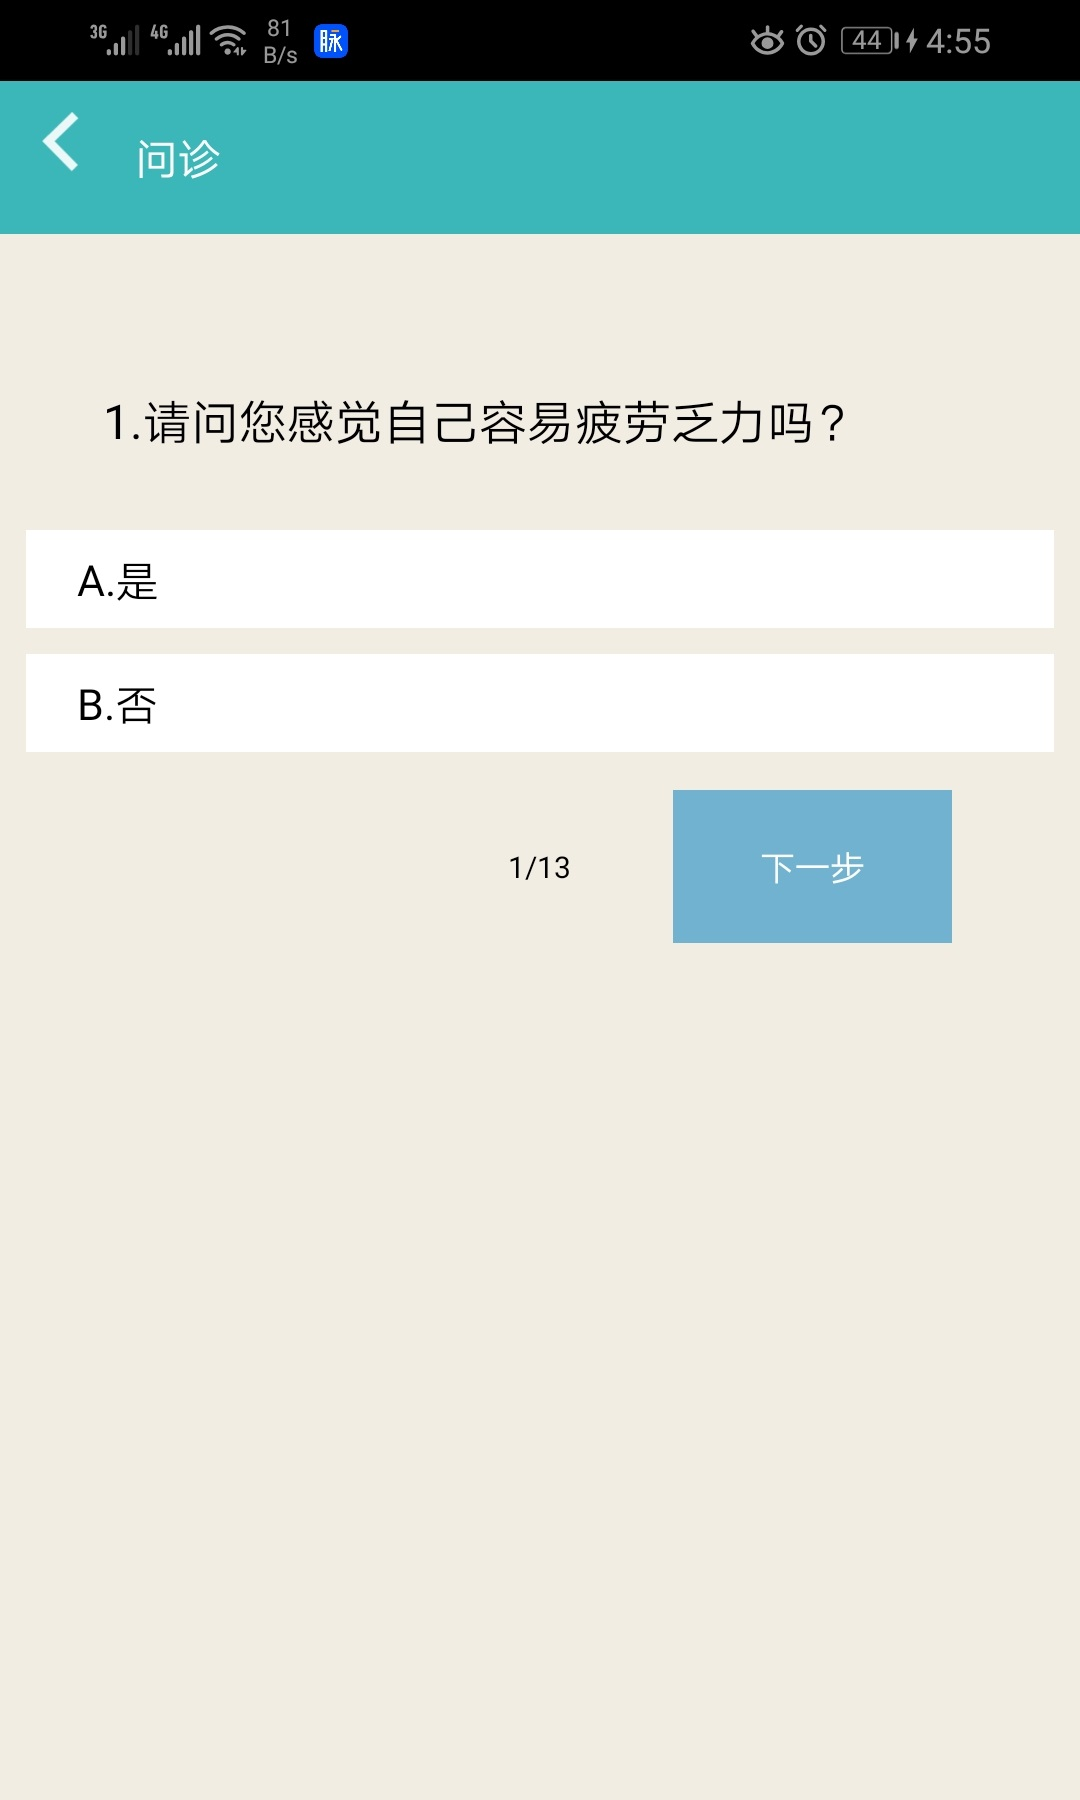
\includegraphics[width=4.5cm]{images/main2.jpg}
    }
    \subfigure[健康报告]{
        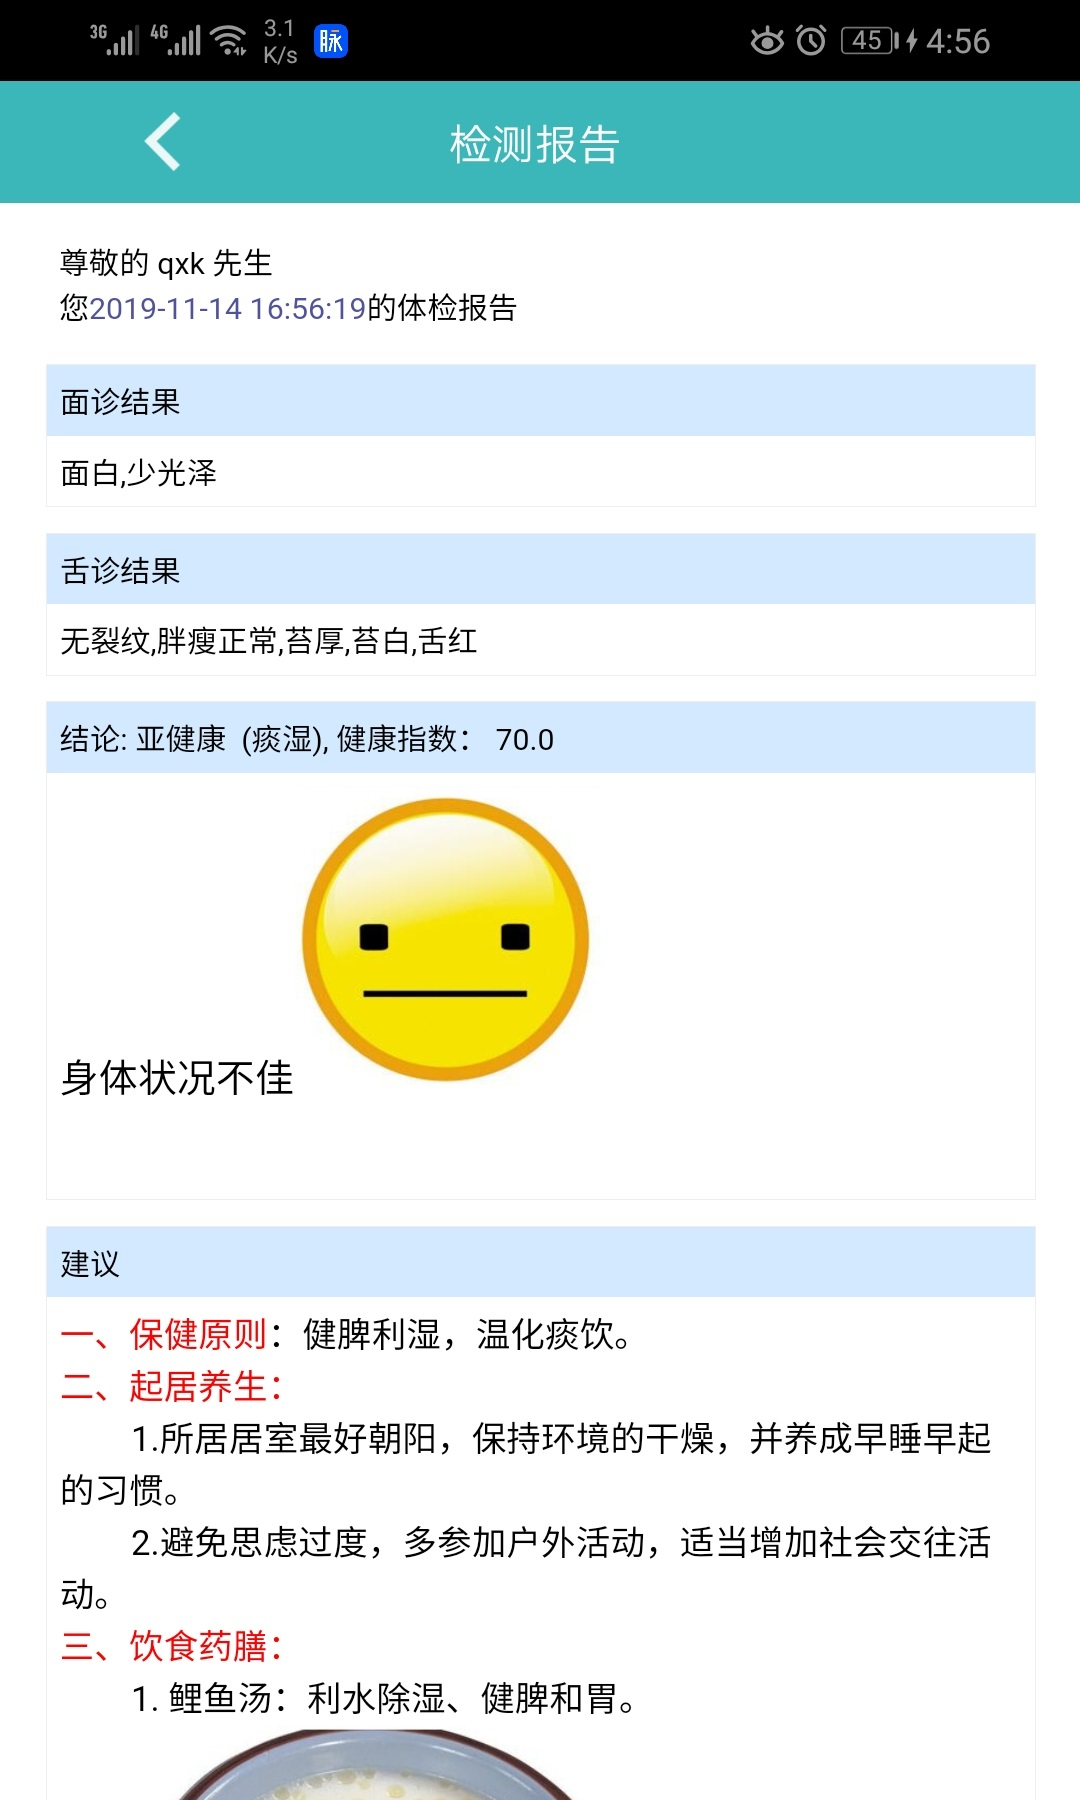
\includegraphics[width=4.5cm]{images/main3.jpg}
    }
    \caption{技术探针的主要界面}
    \label{fig:main}
\end{figure}

云中医应用的主要界面及使用流程如图\ref{fig:main}所示:用户进入诊断页面之后,会看到三个区域:面诊、舌诊、问诊。面诊和舌诊通过拍照或者上传图片完成,问诊是通过依次回答13个问题来完成。依次完成面诊、舌诊、问诊后,系统会给出用户的体质和健康分数,并且给出对应的健康建议。

% 云中医应用\cite{张红凯2018基于舌}的系统设计对设备要求比较灵活,在移动设备、机器人平台上都有对应的产品,其中包括云中医诊断机器人\footnote{http://www.sohu.com/a/135358060\_205169/},云中医智能镜,云中医应用等,但是遗憾的是,云中医虽然功能比较齐全,但是其主要应用场景是社区和诊所等公共环境,缺乏日常健康环境下的用户研究和交互研究。

 

\section{技术探针实验设计}

% 人员招募

\subsection{半结构化深度访谈}

为了尽可能详细地理解用户在日常健康场景下使用面诊技术的各种行为和态度,本文采用半结构化的深度访谈来收集用户数据\cite{DiciccoThe},介绍性的问题大纲如下所示:

\begin{enumerate}
    \item 您的年龄?职业背景?
    \item 您目前健康状况如何?平时感觉身体哪里不舒服吗(慢性病,容易疲劳,关节疼痛等等)?
    \item 您有使用健康状况评估的技术吗?若有,都有哪些技术?平时如何使用的?使用体验如何?
    \item 有看多中医吗?是什么原因看的中医?在哪里看的?效果如何?
    \item 对中医的面诊、舌诊有了解吗?若有,通过什么渠道了解的?
    \item 平时会留意自己的面色,舌苔吗?会留意其他人的面色,舌苔吗?
    \item 您对这个应用感兴趣的点主要在哪里?
\end{enumerate}

本文会根据访谈的深入不断迭代问题大纲,以上只是作为访谈的主题,并不是必须的采访流程。如果在采访中有了新的发现,需要对参与者提到的详细细节进行深入理解,同时在访谈过程中注重客观清晰,避免出现引导性的词语。

\subsection{实验过程}
\begin{figure}[ht]
    \centering
    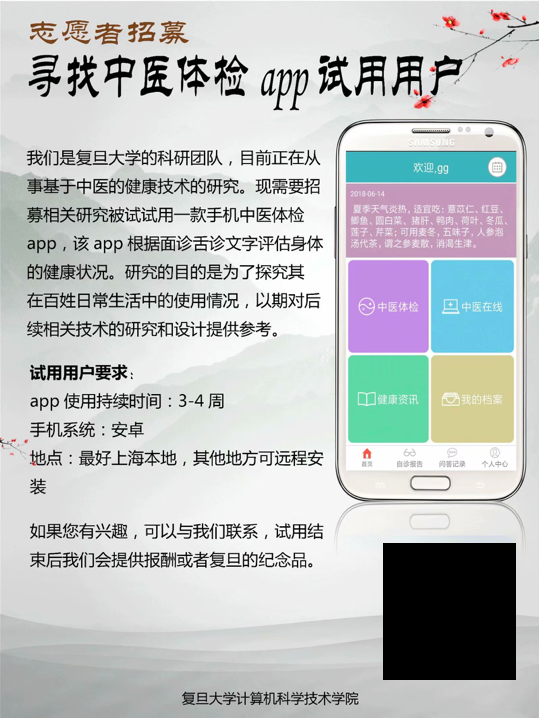
\includegraphics[height=10cm]{images/poster.png}
    \caption{招募海报}
    \label{fig:poster}
\end{figure}

本文通过社交媒体发布海报(如图\ref{fig:poster}所示)招募志愿者参与实验。在被试人员对此应用感兴趣,愿意尝试的前提下,尽量使得招募到的人员在年龄、健康状况、教育背景、工作性质等方面具有多样性。不同的年龄层次可能会导向对健康的不同关注角度(中老年人较为关注的养生知识逐渐在青年群体中流行起来)不同的工作性质使得人们重点关注的身体部位不同(白领普遍关注的肩颈,特殊行业的“职业病”)不同的教育背景使得人们对用技术手段监测健康信息的接受程度也有差异。
    

\begin{table}[htb]
    \centering
    \caption{参与者}
    \begin{tabular}{llll}
          \toprule
          编号 &	性别 &	年龄 &	职业 \\
          \midrule
          参与者1 &	男 &	20多 &	博士生 \\
          参与者2 &	男 &	20多 &	研究生 \\
          参与者3 &	男 &	20多 &	研究生 \\
          参与者4 &	女 &	50多 &	医院护理工 \\
          参与者5 &	男 &	40多 &	办公室职员 \\
          参与者6 &	女 &	40多 &	小学老师 \\
          参与者7 &	女 &	50多 &	办公室职员 \\
          参与者8 &	女 &	19岁 &	本科生 \\
          参与者9 &	男 &	20多 &	办公室职员 \\
          参与者10 &	女 &	40多 &	办公室职员 \\
          \bottomrule
    \end{tabular}
    \label{tab:part}
\end{table}

通过长时间的宣传和参与者筛选,我们最终招募到了10位具有代表性的志愿者,志愿者资料如表\ref{tab:part}所示。
在招募到合适的用户之后,我们会对每一个用户进行一次采访,主要是为了了解用户的基本信息,同时向介绍本文开发的技术探针基本情况和整个实验的基本流程。
    
接下来两周时间,本文让用户回家在日常健康场景下使用技术探针。
在第一星期,本文不对参与者做任何干预,不限制使用方式和地点,尽可能保留原有的使用场景;
为了避免完全获取不到使用数据的特殊情况,到了第二星期,要求用户每天至少使用一次。
在用户使用结束后,我们会采集使用数据,并进行一次结束后的回访,了解用户在使用中遇到的问题和他们的想法,邀请用户一起完成交互设计。


本文希望通过此次调研了解到使用面诊应用的用户群体有哪些?用户期望通过面诊应用来获取哪方面的信息?以及在方便用户日常使用上,有哪些待解决的技术难点?
为了回答这些问题,本文通过分析采访数据进行探索,下面阐述分析过程。

% % 介绍定性研究
% 本用户实验采用的是定性研究方法。定性研究是广泛应用在用户需求调研、人机交互、心理学等领域的研究方法 \cite{崔岩2011统计分析中的定量与定性研究}, 常见的收集数据的方法包括深度访谈、焦点小组访谈、日记、观察法等\cite{李晓凤2006质性研究方法}。

% 研究方法 -> 研究过程->数据采集->数据分析->得出结论


\subsection{数据分析过程}

本文将每个用户对应的采访和回访的录音转录成文字(由于部分访谈时长达到好几个小时,本文采用了转录软件加人工校验的方式),并通过颜色标识用户的身份,最后整理后一共有56页的采访数据,其中部分如图\ref{fig:datas}所示,红色表示采访者,黑色表示被采访者。

\begin{figure}[htb]
    \centering
    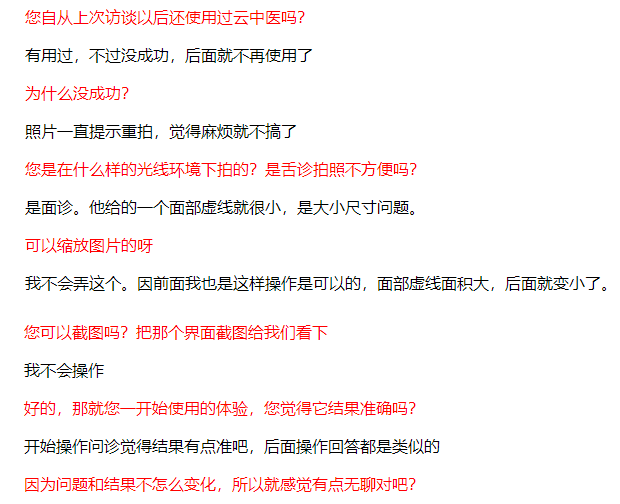
\includegraphics[height=10cm]{images/datas.png}
    \caption{访谈原始数据}
    \label{fig:datas}
\end{figure}



由于采访数据量比较大,本文采用\textbf{主题分析法}(Thematic Analysis)进行数据分析工作,具体分析过程大体如下:

% \begin{table}[htb]
%     \centering
%     \begin{tabular}{|l|l|}
%     \hline
%     一级主题                    & 二级主题        \\ \hline
%     \multirow{3}{*}{可用性}    & 易用性问题       \\ \cline{2-2} 
%                             & 界面问题        \\ \cline{2-2} 
%                             & 交互流程繁琐      \\ \hline
%     \multirow{3}{*}{敏感性}    & 公共场合拍照感到尴尬  \\ \cline{2-2} 
%                             & 设备和环境敏感性    \\ \cline{2-2} 
%                             & 个人隐私        \\ \hline
%     \multirow{3}{*}{情绪与信赖}   & 诊断模型细节不可见   \\ \cline{2-2} 
%                             & 缺乏对结果的评估机制  \\ \cline{2-2} 
%                             & 不好的结果导致消极情绪 \\ \hline
%     \multirow{2}{*}{自适应性}   & 总是问同样的问题    \\ \cline{2-2} 
%                             & 结果无变化     \\ \hline
%     \multirow{2}{*}{对结果的理解} & 不了解专业术语     \\ \cline{2-2} 
%                             & 诊断结果不够直观    \\ \hline
%     \end{tabular}
%     \caption{抽取的部分主题}
%     \label{tab:theme}
% \end{table}


\begin{enumerate}
    \item 数据预处理。对访谈记录中的数据进行删减,只提取关心的内容。如图\ref{fig:datas}中,\myfont{照片一直提示重拍,觉得麻烦就不搞了}、\myfont{问题和结果不怎么变化,所以就感觉有点无聊}等数据是我们关注的数据,将其提取出来。

    \item 关键词提取。对保留的内容进行分类,从中提取关键词。然后再根据关键词提取出新的分类,由新分类返回到步骤(1)循环提取相关的内容。例如通过\myfont{问题和结果不怎么变化,所以就感觉有点无聊}中\myfont{无聊}的关键词,我们可以回到原始数据提取\myfont{无聊}的原因是\myfont{结果无变化}等新关键词。
    
    \item 多次迭代。反复迭代步骤(1)和步骤(2),直到无法提取出新的内容和新的关键词为止。

    \item 主题提取。主题是对关键词所反映的内容模型的抽象化,在访谈数据中重复出现并且具有共通性。通过归纳主题能够将提取出来的关键词联系起来对访谈的内容进行解释。
    例如通过以上步骤,本文可以由上述关键词归纳出日常健康场景下面诊技术需要解决\myfont{自适应性}的问题,缺乏通过自适应用户数据吸引用户持续使用的机制等。

    \item 回访验证。获取基本主题以后,一方面为了避免主观意见对资料与主题的相关性造成干扰,另一方面由于本文主要资料来源为用户的定性访谈转录出来的文字,可能会因为发音以及转录质量的问题引入错误数据。
因此本文根据主题分析法得到的基本主题,对参与者进行了进一步的以基本主题为中心深入访谈,已验证访谈数据的准确性,同时通过基本主题进行发散进一步得到更多的主题和佐证资料。
\end{enumerate}


\section{日常健康场景下面诊技术的应用问题}

在研究中本文发现,在日常健康场景中遇到了各种问题和阻碍,大部分用户在使用几次之后就没有坚持继续使用。总的来说,通过技术探针本文发现主要有以下几个方面:

\subsection{自适应性问题}

日常环境和诊所环境不同,日常环境下需要用户长期使用。但是,大部分的参与者在使用云中医一到两次后就不再使用了,其中一个重要的原因就是云中医缺乏自适应性的能力。

比如参与者1在采访中指出:\myfont{无论我什么时候拍照,它都是问我同样的问题,我会感觉很无聊。}
同样,参与者2说:\myfont{每次都重复地检查很枯燥。}参与者6解释了她不继续用云中医的原因:\myfont{一个人的健康状况,在短时间内的变化不会太大,所以我就没一直用了。}
而参与者7虽然在持续使用,但是也不愿意每次看到相同的信息:\myfont{它每次都给我相同的健康结果,我怀疑它的准确性。}

参与者在提出问题的同时,也给了对应提高系统自适应性的建议,主要体现在两个方面:

\subsubsection{对用户信息的自适应性}

从调研反馈来看,本文发现因为云中医在问诊的时候,一直问用户同样的问题,而实际情况是短期内来说,大部分问题的答案是不会发生改变的,这样缺乏用户信息的自适应性会让用户使用起来觉得很繁琐。

在这次的用户研究过程中,在诊断应用的场景下,本文发现用户强烈希望系统能够记住他们的用户信息并对下一次诊断进行相应的调整。
比如一些参与者抱怨说每次去回答问诊的问题非常地繁琐,参与者2说道:\myfont{问诊那一部分设计地不好,每次问题都是固定的,而且太笼统了。},然后他建议这些问题应该更加个性化:\myfont{我认为问诊的问题可以根据之前问的问题更加地具体。}
参与者10则希望系统能够追踪用户的健康状况:\myfont{我希望它有后续的追踪过程,不仅可以评估当天的健康状况,也可以在接下来的几天内,跟踪健康问题并动态地调整建议。}
参与者3也有类似的想法:\myfont{目前系统只有诊断的功能,我希望系统能够接受用户的反馈,比如记录系统给出的健康建议是否有效,这样可以调整健康建议的结果。}

\subsubsection{对环境信息的自适应性}

系统给出的养生建议也是固定的,并没有考虑到用户当前的工作状态和环境因素。中医认为,与环境变化和谐相处对于保持健康很重要,特别是在季节变化的时候,即中医中所说的\myfont{天人合一}。

参与者6建议:\myfont{养生建议应该更加丰富一些,比如考虑季节和节气的变化。}
参与者10希望系统能健康建议和当前天气综合考虑:\myfont{那么热的天气叫我出去运动? 它应该考虑到我个人的健康情况和当前的天气情况。}


\subsection{实用性问题}
在调研过程中,本文发现并不是所有的参与者都能接受健康报告的结果,主要原因有以下两个方面:

\subsubsection{中医术语理解的问题}

技术探针在用户界面中文字使用的是标准的中医术语。和平时就医环境不同的是,在日常环境下,用户在使用的时候,周围是没有专业的医生可以询问的,因此通俗易懂的解释中医术语是非常重要的。
在调研过程中本文发现很多参与者很难理解系统给出的健康报告,特别是在年轻群体中,新一代年轻人对中医的接受程度比较低,这个问题就更加严重。
参与者2是在读研究生,对健康报告的里“气”的概念就不是很了解,他提到:\myfont{我对中医知之甚少,它说我气虚,但是什么是气虚我都不知道……}

参与者8也觉得自己对中医知识了解有限,对结果不是很理解:\myfont{分数下面有提到五脏的概念,但是其实我连五脏指的是哪五个器官不是很清楚,可能包括肝脏、心脏和肾脏?}
虽然中医在中国的历史悠久,但是并不是所有的人都清楚中医中的常见概念。 如果系统是设计给普通用户日常使用的话,就需要考虑到用户的中医知识素养了。

解决此类问题的方法之一,是把中医术语和常见的词语进行关联。比如参与者1遇到这样一个例子:\myfont{我今天感冒了,但是系统却没有提示我感冒了,只是说我气血不畅,它为什么不直接告诉我感冒或者风寒呢?}

另一个解决方法则是通过更加生动的方式进行介绍,比如视频图片等。还是参与者1,他说:\myfont{健康建议里的按摩,可能直接给出一个按摩的视频,而不是只有文字和图片,有一个视频跟着做的话会更好。}

参与者还提出可以通过提供学习的机制,让用户了解晦涩的中医术语。
事实上在调研过程中,就有参与者把云中医当作一个学习中医养生的工具,例如参与者10提到:\myfont{我认为系统可以提供更加宽泛的养生知识,而不只是健康建议。我对健康建议中的穴位按摩就很感兴趣。}

\subsubsection{养生建议合理性}

不同职业的用户,日常的空余时间是不同的。空余时间是否充裕,是影响用户实践养生建议的关键。因此系统给出的养生建议,特别是需要花费较长时间的按摩熬粥之类大的养生活动,需要合理考虑用户的日常空余时间。

比如参与者2就指出:\myfont{作为一个住在没有厨房的公共宿舍的学生,养生建议中的食疗就是不切实际的。我不会做饭,而且有些食物用的材料太贵了,超出了我的承受范围。}
参与者9是一位刚参加工作的算法工程师,每天8点才下班,他反馈说:\myfont{我基本没有什么时间熬粥或者煎药了。}参与者7表示:\myfont{每天都进行穴位按摩太费时间了,我坚持不下来。}

\subsection{敏感性问题}

\subsubsection{文化敏感性}


舌诊的时候,需要用户伸出舌头进行拍照,这个过程可能会给用户带来烦恼。
在中国文化中,伸出舌头可以表示厌恶或者无礼,并且大部分中国人是比较传统的。因此在很多情况下,在公众场合伸出自己的舌头被认为是不合适的。大部分参与者表示伸出舌头会让他们感到尴尬,或者是害怕自己因为伸出舌头在无意间冒犯到别人。
如参与者1认为,伸出舌头拍舌头的照片是很不雅的。参与者3表示自己在和别人拍照的时候都会感到紧张,使用云中医时都是私下使用。特别是年轻人来说,参与者8直白地指出伸出舌头这个动作太丑了,她只会在私人空间下使用应用,她甚至调侃说:\myfont{我觉得这个软件是太有意思了,因为它有拍舌头的各种照片,完全就是收集丑照的一大利器。}

不过有趣的是,对于年纪稍大的参与者或者老年人来说,对于伸出舌头进行诊断并不是非常在意。例如参与者10说:\myfont{我并不觉得尴尬,因为这是一种诊断。},参与者4对这一现象解释说:\myfont{对于像我这样的年纪的人来说,就不那么在乎了}。 

总而言之,这个发现提醒了我们文化敏感性限制了面诊类应用的日常使用范围。


\subsubsection{技术敏感性}


由于模型的计算需要对面部舌部图片进行颜色特征的提取,使其对外部因素如光照和手机摄像头的质量会更加敏感,已经严重影响了部分用户的使用。
参与者7在系统一次又一次提示检测不到照片中的人脸之后选择了放弃:\myfont{照片一直提示重拍,觉得麻烦就不用了。}
参与者8还特别反映了自己用的是某品牌手机,拍照会受到相机自带美颜算法的影响:\myfont{但是你需要考虑,我现在用的手机是某品牌手机,它的相机自带美颜的功能。你把照片传过去,那准确率不就下降了吗?}

由于目前技术的问题,环境和设备的多样性不仅可能降低最终结果的准确率,甚至会影响用户的正常使用。因此,在离开诊所环境下严格统一的光线和设备条件之后,将面诊应用日常环境下,从技术的层面来讲,需要考虑更多的因素。
或者说,在技术无法改进的前提下,应该如何设计系统来屏蔽这些环境因素和设备的差异性,也是一个需要考虑的问题。

\subsubsection{社交敏感性}


虽然有几位参与者希望分享它们的健康结果给其他人作为相互学习的机会,但是他们同时也担心因为涉及到面部照片和个人健康信息,可能会导致隐私泄露的问题。
如参与者10讨论了可接受的分享的范围:\myfont{我觉得,比如说有什么症状我可以分享。比如说我今天有哪里不舒服了,得到了哪个专家的帮助,然后经过一段调理,我觉得我有好转了。但是有些可能关系到自己个人隐私的事情,我还是有点不愿意分享的。}

大部分参与者虽然不太愿意分享自己的诊断结果,但是如果将分享的范围限制在家庭或者医生圈子等可信任的人之内的话,他们表示可以接受。不过有趣的是,本文发现和其他社交分享类应用不同的是,对于家人来说,他们更加愿意分享给陌生人,因为分享给家人的话可能会引起家人不必要的担心,如参与者3表示:\myfont{其实我觉得分享的话更倾向的是和一些陌生人分享,如果和亲人分享的话,就觉得反而让他们,但是反而觉得是一种负担,如果和陌生人分享,就会觉得这是一个这一个交流的,就是一个也算是一个社交的一种方式吧,同时也能提高自己的健康知识。}


\subsection{信赖与情绪的问题}
关于用户对于日常面诊技术的态度,本文在本次用户研究过程中也进行了探讨。在调研过程中,本文发现许多参与者对产生的结果持怀疑态度,从而导致他们不信赖系统。
例如当参与者发现系统给出的健康分数较低时,他们不会去反思是不是自己的生活方式不够健康或者其他原因,而是质疑系统的准确性。参与者3认为系统给他的低分数是因为系统的缺陷:\myfont{看到它结果不好的时候,我就第一反应就觉得这个应用有问题。就是其实我本身并没有不舒服,但是它打的分很低。我就会想他是不是它面部检测的这个效果不好,还有它这个诊断的这一个整个的正确率也不好。}

在没有其他的评估机制验证结果有效性的前提下,参与者会倾向与根据自己的感觉去判断。一方面,如果结果和自己情况不符合,他们会产生不信任的情绪甚至放弃使用,如参与者2透露:\myfont{也不是很不舒服,我觉得我自己还挺好的,还是就老给我打那么低的分……我就真的我觉得我还没有那么严重,就不想用它了。};另一方面,他们认为结果是可靠地就会促进他们继续使用,如参与者5说:\myfont{基本和我医院看的说法差不多……我觉这个做的很好,符合我的实际情况。}但是需要注意的是,调研过程中,参与的的个人感受和看法可能并不能反映他们真实的健康状况。

此外,本文通过分析访谈数据还发现,系统的结果会对使用者的情绪产生影响,特别是分数很低的时候。例如对于参与者8来说,很低的分数对于她来说是不能接受的,因为她已经坚持健康作息很长一段时间了:\myfont{也不是吧,就是感觉受到打击了吧,因为那个时候我还是生活得非常健康的。期末考试那段时间我非常不健康作息的时候都能测到89,现在结果却这么低,真是见了鬼了。}这也验证了之前的研究\cite{Toscos2013Designing}的结论,健康评测系统会引发用户的消极情绪,特别是当系统给出负面结果的时候需要非常注意。

一些参与者提出,他们需要了解结果背后的原理机制,以便知道如何对结果进行评估。如参与者1认为知道结果是如何得出的很重要:\myfont{它需要告诉我它的数据是怎么来的,否则我不太相信}。而另一位计算机专业的参与者则
希望通过了解背后的算法原理来判断它是否可靠:\myfont{我认为这个背后的模型有些过于简单。通过一些基本的面色、舌苔等指标的规则组合做出对健康的评判,似乎很难让人相信能非常贴切、准确地反映自己的健康状况。在图像方面感觉需要更复杂的模型来对健康状况和面色、舌苔等之间的关系进行发现,这样才使我信服,确实这个系统里的中医有其专业性,能对我的健康提出有益的建议。一个经验丰富的老中医可能需要自己一生的行医积累,才能从表面相同的症状分析出背后不同的病源,有针对性的开方子医治;从计算机专业讲,这可能需要用深度学习的复杂模型才能接近这个过程及达到的效果。}很明显,将系统背后的原理和数据暴露给用户是帮助用户评估系统可靠性的一种方法。

\section{日常健康场景下面诊技术的设计策略}
设计策略与设计方案不同,其作用主要指明设计的方向,不包含具体实现,主要为后续系统实现提供指导。

通过本次用户研究,本文发现在日常使用场景下,基于人脸识别技术的健康应用存在着大量待解决的设计方面的问题,而且大多数问题是和使用了面部图片进行面诊相关。
为了帮助更好地设计日常面诊应用,本文总结之后认为日常健康场景下的面诊系统系统应该遵循以下的设计策略。

\subsection{支持可持续使用}
在以往鼓励健康生活类交互技术的研究中,用户持续使用一直是一个重要的问题\cite{Clawson2015No, Epstein2016Beyond}。在本次研究中,也出现过大量的用户不继续使用的情况。
在所有的原因中,最重要的因素是没有出现新的东西,如每次都要拍脸,拍舌头,回答同样的问题,系统给出的也是同样的结果等。

本次实验的环境是要求用户每天使用一次,系统每次都是问同样的问题,然后用户健康状况变化不大的话,也会给出类似同样的结果。本次数据表明,用户很快会对系统失去兴趣。

一方面,基于这个发现,本文建议在设计此类应用的时候,把用户分为两类分别讨论:

\begin{itemize}

    \item 对于健康状况有变化的用户,系统应该允许用户跳过某些步骤,只让用户回答这次不同的地方,或者突出显示出本地和上次记录中出现变化的部分。这样能够减少用户每次诊断的时间,同时用户能追踪自己的健康变化。

    \item 对于健康状况没有变化的用户,可以加入上下文的信息让结果有稍微的变化。例如加入天气和气候的因素,给出用户不同的建议。这样不仅增加了用户对结果的新鲜感,也能让用户学习到天气和气候相关的知识。

\end{itemize}

另一方面,可以将健康知识以推送的方式显示给用户。如果知识库特别大的话,可以一次推送一部分的健康知识,这样也能增加系统的可变性,以此支持用户的持续使用。

\subsection{系统可解释性}

和其他成熟的商业健康产品,如血压计,血糖仪不同,基于人脸的健康诊断技术仍是一项新兴的非常不成熟的技术。因此从相对权威的应用场景如诊所,转移到日常环境下时,系统的可靠性会被经常受到质疑。

本次研究数据表明,系统的可靠性或者说信任度也是影响用户继续使用的关键因素。对于本次交互研究使用的技术探针云中医,虽然它是利用大量的数据训练而成,但用户在使用的时候,并不知道它背后的技术原理,只能通过自己的直觉来判断系统的准确性。

基于这个发现,本文建议系统在设计的时候,将背后的技术原理和开发背景暴露给用户,从而增加用户的理解度,让用户更好地对结果进行评估。

当然,对于当前的人工智能应用来说,系统不是万能的,总是会存在误判。此类应用的设计目的,并不是为了取代专业的医生进行诊断,而且很多的因素也会影响最终的结果,如拍照时背景光线的强度,设备相机的分辨率,截取图片的区域等对结果影响很大。在进行可解释设计的时候,也可以把系统的局限性告知给用户。

\subsection{日常可用性}
基于人脸的诊断应用的特殊性在于,在这个过程中,用户需要拍脸和拍舌头。对于拍脸来说,在中国比较传统的社会环境下,大部分人是比较害羞的,没有拍脸的习惯,特别是在日常的场景下,在公共场合下拍脸;对于拍舌头来说,在别人面前伸出舌头拍照,是一件很不雅观的事情,影响个人形象。

正如本次实验数据所示,大部分参与者在使用的时候,都是在周围没有人的时候,或者在宿舍中进行。也就是说,让用户去拍脸拍舌头从技术上讲是没有实现难度,但是从社会从文化上来说,有些用户是难以接受的。另一方面,大部分用户反馈每次都要重新完成之前做过的操作,非常繁琐。比如用户每次都需要回答13个问诊的问题,而大部分人在短时间内,这些问题的答案并不会发生变化。

此外,在目前的互联网环境下,用户的可能会觉得自己的自拍有可能会导致隐私泄露的问题。用户在使用的时候会考虑到自己拍脸导致隐私泄露而拒绝使用。

基于上面的讨论,本文建议在设计的时候,在不影响系统使用的情况下,尽可能把面诊舌诊设计成系统中可选的选项,允许用户跳过某些步骤。

不过,在本次研究中,也有用户发表了完全不同的想法:有的用户愿意分享自己的面诊照片,认为这是一种和类似人群交流学习的机会。

\section{本章小结}


本章介绍了通过技术探针的方法,招募了一群参与者,设计并对参与者进行了深度访谈。
通过分析访谈数据,发现了日常健康场景下中医面诊应用的潜在使用场景,以及目前存在的的自适应性、实用性、敏感性等问题,
同时从设计的角度给出了支持可持续使用、系统可解释性,日常可用性等改进思路,为日常健康场景下的面诊应用的设计提供了改进思路。


